\documentclass[11pt,paper=a4,answers]{exam}
\usepackage{graphicx,lastpage}
\usepackage{upgreek}
\usepackage{censor}
\usepackage{gensymb}
\usepackage{amsmath}
\usepackage{multicol}
\usepackage{enumitem}
\usepackage{tasks}
\usepackage{adjustbox}
\usepackage{xcolor}
\usepackage{tfrupee}
\setlength{\voffset}{0.25in}
\usepackage{tabularx}
\newcolumntype{Y}{>{\centering\arraybackslash}X}
%==============================================================
% Customise Non-Essential Packages Below
% =============================================================
\usepackage[most]{tcolorbox}
\usepackage{eso-pic}
\usepackage{tikz}
\AddToShipoutPictureBG{%
\begin{tikzpicture}[remember picture,overlay]
\foreach \x in {-8,-4,0,4,8,12,16,20}
\foreach \y in {-8,-4,0,4,8,12,16,20} {
\node[opacity=0.05,rotate=45,anchor=center] at ([xshift=\x cm,yshift=\y cm]current page.center) {%
\begin{minipage}{2cm}
\centering
\includegraphics[width=2cm]{images/logo_black.png}\\
\small preppeo.com
\end{minipage}%
};
}
\end{tikzpicture}%
}
\printanswers

%==============================================================
% Customise Non-Essential Packages Above
% =============================================================
\definecolor{svgray}{rgb}{0.90, 0.90, 0.90}
\graphicspath{{images/}}

\usepackage[normalem]{ulem}
\renewcommand\ULthickness{1pt}   %%---> For changing thickness of underline
\setlength\ULdepth{3.5ex}%\maxdimen ---> For changing depth of underline
\renewcommand{\baselinestretch}{1}
\chead{
\includegraphics[scale=0.1,height=2cm ]{logo.png}
}
\pagestyle{empty}

\pagestyle{headandfoot}
\headrule
\cfoot{W: https://preppeo.com; M: +91-8130711689}

\begin{document}
%==============================================================
% Customise Question paper details below this
% =============================================================
\begin{center}
    \centering
    \renewcommand{\arraystretch}{1.5}
    \begin{tabularx}{\textwidth}{YYY}
    & \normalsize\bf{{\Large{{Quant}}}} & \\
    By Preppeo & \normalsize\bf{{alg\_sat\_easy\_018}} & SAT\\
    \normalsize{{\textbf{{Algebra}} }} & \normalsize{{\textbf{{Linear equations, systems, inequalities }} }} & \normalsize{{\textbf{{Solving Linear Equations}} }} \\
    \end{tabularx}
\end{center}
\par\noindent\rule{\textwidth}{1pt}
% =============================================================
% Customise Question paper details above this
% =============================================================

\begin{questions}
\pointsinrightmargin
\pointsdroppedatright
\marksnotpoints
\pointpoints{mark}{marks}
\pointformat{\boldmath\themarginpoints}
\bracketedpoints

% =============================================================
% Question Begin
% =============================================================

\section*{SAT Algebra - Practice Set 1 (Easy)}

% Q1: Based on Point (8,2) logic
\question
The point $(5, -3)$ in the $xy$-plane is a solution to which of the following systems of inequalities?
\begin{tasks}(2)
\task $x > 0$ and $y > 0$
\task $x > 0$ and $y < 0$
\task $x < 0$ and $y > 0$
\task $x < 0$ and $y < 0$
\end{tasks}

\begin{solution}
To find the correct system of inequalities, we evaluate the signs of the given coordinates $(5, -3)$.
\vspace{5pt}
\begin{center}
The $x$-coordinate is $5$, which is positive ($5 > 0$).
\vspace{5pt}
The $y$-coordinate is $-3$, which is negative ($-3 < 0$).
\end{center}
\vspace{5pt}
The point satisfies the conditions where $x$ is positive and $y$ is negative.
\vspace{5pt}
Answer: \colorbox{yellow!100}{B}
\end{solution}

\vspace{1cm}

% Q2: Based on Airplane Speed logic
\question
A delivery drone's altitude during a specific mission varied between $80$ meters and $120$ meters. Which inequality best represents this situation, where $a$ is the altitude in meters?
\begin{tasks}(2)
\task $a \leq 40$
\task $a \geq 120$
\task $80 \leq a \leq 120$
\task $a \leq 80$
\end{tasks}

\begin{solution}
The altitude $a$ is restricted to a range with a minimum of $80$ and a maximum of $120$.
\vspace{5pt}
\begin{center}
This is represented by $a$ being greater than or equal to $80$ AND less than or equal to $120$.
\end{center}
\vspace{5pt}
The compound inequality $80 \leq a \leq 120$ captures the entire interval of the drone's mission.
\vspace{5pt}
Answer: \colorbox{yellow!100}{C}
\end{solution}

\vspace{1cm}

% Q3: Based on Red Beads logic - ADDED TIKZ
\question
A juice company produces a blend where $40\%$ is apple juice and $10\%$ is grape juice. The total volume of these two juices must be at least $300$ liters.
\begin{center}
\begin{tikzpicture}[scale=0.8]
\draw[thick] (0,0) rectangle (4,2.5);
\fill[red!20] (0,0) rectangle (2.5,2.5);
\fill[purple!20] (2.5,0) rectangle (4,2.5);
\node at (1.25,1.25) {\small $40\% x$};
\node at (3.25,1.25) {\small $10\% y$};
\node[below] at (2,-0.2) {\small Total $\geq 300$ Liters};
\end{tikzpicture}
\end{center}
Which inequality represents this relationship, where $x$ is the volume of the first container and $y$ is the volume of the second?
\begin{tasks}(2)
\task $0.4x + 0.1y \geq 300$
\task $0.1x + 0.4y \leq 300$
\task $40x + 10y \geq 300$
\task $0.4x + 0.1y < 300$
\end{tasks}

\begin{solution}
We convert the percentages to decimals to find the actual volume contributed by each container.
\vspace{5pt}
\begin{center}
Apple juice volume $= 0.40x$ and Grape juice volume $= 0.10y$.
\vspace{5pt}
The phrase "at least $300$" implies a sum that is greater than or equal to $300$.
\end{center}
\vspace{5pt}
Therefore, the correct inequality is $0.4x + 0.1y \geq 300$.
\vspace{5pt}
Answer: \colorbox{yellow!100}{A}
\end{solution}

\vspace{1cm}

% Q4: Based on Line n intercept/slope logic - ADDED TIKZ
\question
Line $p$ is graphed in the $xy$-plane and passes through the intercepts shown below.
\begin{center}
\begin{tikzpicture}[scale=0.5]
\draw[step=1cm,gray!20,very thin] (-5,-1) grid (2,6);
\draw[thick,->] (-5,0) -- (2,0) node[right] {\tiny $x$};
\draw[thick,->] (0,-1) -- (0,6) node[above] {\tiny $y$};
\filldraw[black] (-3,0) circle (3pt) node[below left] {\tiny $(-3,0)$};
\filldraw[black] (0,5.33) circle (3pt) node[right] {\tiny $(0, \frac{16}{3})$};
\draw[ultra thick, blue] (-4,-1.77) -- (0.5,6.22);
\end{tikzpicture}
\end{center}
What is the slope of line $p$?
\begin{tasks}(2)
\task $\frac{9}{16}$
\task $\frac{16}{9}$
\task $\frac{3}{16}$
\task $\frac{16}{3}$
\end{tasks}

\begin{solution}
The slope $m$ is determined by the vertical change divided by the horizontal change between $(-3, 0)$ and $(0, \frac{16}{3})$.
\vspace{5pt}
\begin{center}
$m = \dfrac{y_2 - y_1}{x_2 - x_1} = \dfrac{\frac{16}{3} - 0}{0 - (-3)}$
\vspace{5pt}
$m = \dfrac{\frac{16}{3}}{3} = \dfrac{16}{3} \times \dfrac{1}{3} = \dfrac{16}{9}$
\end{center}
\vspace{5pt}
Answer: \colorbox{yellow!100}{B}
\end{solution}

\vspace{1cm}

% Q5: Based on Perpendicular line logic
\question
Line $k$ is defined by $y = \frac{2}{3}x + 5$. Line $j$ is perpendicular to line $k$. What is the slope of line $j$?
\begin{tasks}(2)
\task $\frac{2}{3}$
\task $-\frac{2}{3}$
\task $\frac{3}{2}$
\task $-\frac{3}{2}$
\end{tasks}

\begin{solution}
Perpendicular lines have slopes that are negative reciprocals of one another.
\vspace{5pt}
\begin{center}
The slope of line $k$ is $m = \frac{2}{3}$.
\vspace{5pt}
The negative reciprocal of $\frac{2}{3}$ is $-\frac{3}{2}$.
\end{center}
\vspace{5pt}
Answer: \colorbox{yellow!100}{D}
\end{solution}

\vspace{1cm}

% Q6: Based on Table Equation logic
\question
\begin{center}
\begin{tabular}{|c|c|}
\hline
$x$ & $y$ \\ \hline
0 & 10 \\ \hline
1 & 7 \\ \hline
2 & 4 \\ \hline
\end{tabular}
\end{center}
The table shows a linear relationship between $x$ and $y$. Which equation represents this relationship?
\begin{tasks}(2)
\task $y = -3x + 10$
\task $y = 3x + 10$
\task $y = -3x + 7$
\task $y = -10x + 3$
\end{tasks}

\begin{solution}
Identify the $y$-intercept when $x=0$, which is $10$.
\vspace{5pt}
\begin{center}
Find the slope by observing the change: as $x$ increases by $1$, $y$ decreases by $3$.
\vspace{5pt}
Slope $m = -3$.
\end{center}
\vspace{5pt}
Plugging these into $y = mx + b$ gives $y = -3x + 10$.
\vspace{5pt}
Answer: \colorbox{yellow!100}{A}
\end{solution}

\vspace{1cm}

% Q7: Based on Sweater/Shirt purchasing logic
\question
The equation $30x + 15y = 120$ represents the number of notebooks, $x$, and pens, $y$, a student bought for $\$120$. If the student bought $2$ notebooks, how many pens did they buy?
\begin{tasks}(2)
\task $2$
\task $4$
\task $6$
\task $8$
\end{tasks}

\begin{solution}
Substitute $x = 2$ into the given linear equation to solve for $y$.
\vspace{5pt}
\begin{center}
$30(2) + 15y = 120$
\vspace{5pt}
$60 + 15y = 120$
\vspace{5pt}
$15y = 60 \implies y = 4$
\end{center}
\vspace{5pt}
Answer: \colorbox{yellow!100}{B}
\end{solution}

\vspace{1cm}

% Q8: Based on Petting Zoo logic
\question
A museum sells child tickets for $\$10$ and adult tickets for $\$20$. On Saturday, the museum sold $150$ tickets total and earned $\$2,200$. Which system of equations represents this, where $c$ is child tickets and $a$ is adult tickets?
\begin{tasks}(1)
\task $c + a = 150$ and $10c + 20a = 2,200$
\task $c + a = 2,200$ and $10c + 20a = 150$
\task $10c + 20a = 150$ and $c + a = 150$
\task $20c + 10a = 150$ and $c + a = 2,200$
\end{tasks}

\begin{solution}
The first equation must represent the total quantity of tickets sold ($150$).
\vspace{5pt}
\begin{center}
$c + a = 150$.
\vspace{5pt}
The second equation must represent the total monetary value earned ($\$2,200$).
\vspace{5pt}
$10c + 20a = 2,200$.
\end{center}
\vspace{5pt}
Answer: \colorbox{yellow!100}{A}
\end{solution}

\vspace{1cm}

% Q9: Based on Graph Solution logic
\question
\begin{center}
\begin{tikzpicture}[scale=0.6]
\draw[help lines, color=gray!30, step=1] (0,0) grid (8,8);
\draw[thick,->] (0,0) -- (8.5,0) node[right] {\tiny $x$};
\draw[thick,->] (0,0) -- (0,8.5) node[above] {\tiny $y$};
\draw[ultra thick, red] (0,6) -- (6,0);
\draw[ultra thick, blue] (0,2) -- (6,8);
\filldraw[black] (2,4) circle (3pt);
\end{tikzpicture}
\end{center}
The graph of a system of linear equations is shown. What is the solution $(x, y)$ to the system?
\begin{tasks}(2)
\task $(2, 4)$
\task $(4, 2)$
\task $(3, 3)$
\task $(1, 5)$
\end{tasks}

\begin{solution}
The solution to the system is the point $(x, y)$ where the two lines intersect.
\vspace{5pt}
\begin{center}
Looking at the grid, the intersection point is located $2$ units to the right of the $y$-axis and $4$ units above the $x$-axis.
\end{center}
\vspace{5pt}
The coordinates are $(2, 4)$.
\vspace{5pt}
Answer: \colorbox{yellow!100}{A}
\end{solution}

\vspace{1cm}

% Q10: Based on Substitution logic
\question
$y = 3x + 2$ \\
$x = 4$ \\
What is the solution $(x, y)$ to the given system of equations?
\begin{tasks}(2)
\task $(4, 10)$
\task $(4, 14)$
\task $(14, 4)$
\task $(4, 12)$
\end{tasks}

\begin{solution}
We are given that $x = 4$, so we substitute this value into the first linear equation to find $y$.
\vspace{5pt}
\begin{center}
$y = 3(4) + 2$
\vspace{5pt}
$y = 12 + 2 = 14$
\end{center}
\vspace{5pt}
The solution is $(4, 14)$.
\vspace{5pt}
Answer: \colorbox{yellow!100}{B}
\end{solution}

\section*{SAT Algebra - Practice Set 2 (Easy)}

% Q1: Based on Linear Graph Solution
\question
A system of two linear equations is graphed in the $xy$-plane below.
\begin{center}
\begin{tikzpicture}[scale=0.5]
\draw[step=1cm,gray!20,very thin] (-2,-2) grid (10,10);
\draw[thick,->] (-2,0) -- (10.5,0) node[right] {\tiny $x$};
\draw[thick,->] (0,-2) -- (0,10.5) node[above] {\tiny $y$};
\foreach \x in {2,4,6,8,10} \node[below] at (\x,0) {\tiny \x};
\foreach \y in {2,4,6,8,10} \node[left] at (0,\y) {\tiny \y};
\draw[ultra thick, blue] (-1,1) -- (8,10);
\draw[ultra thick, red] (1,10) -- (6,0);
\filldraw[black] (4,6) circle (3pt) node[above right] {\tiny $(4,6)$};
\end{tikzpicture}
\end{center}
Which of the following points is the solution to the system of equations?
\begin{tasks}(2)
\task $(4, 6)$
\task $(6, 4)$
\task $(0, 2)$
\task $(5, 2)$
\end{tasks}

\begin{solution}
The solution to a system of equations corresponds to the point of intersection on a graph.
\vspace{5pt}
\begin{center}
By inspecting the grid, the two lines intersect exactly at $x = 4$ and $y = 6$.
\end{center}
\vspace{5pt}
Therefore, the ordered pair $(4, 6)$ satisfies both equations simultaneously.
\vspace{5pt}
Answer: \colorbox{yellow!100}{A}
\end{solution}

\vspace{1cm}

% Q2: Based on 2x value logic
\question
$x + 5 = -3y + 12$ \\
$x - 5 = 3y + 8$ \\
The solution to the given system of equations is $(x, y)$. What is the value of $3x$?
\begin{tasks}(2)
\task $10$
\task $20$
\task $30$
\task $40$
\end{tasks}

\begin{solution}
We can solve this system using the elimination method by adding the two equations together.
\vspace{5pt}
\begin{center}
$(x + 5) + (x - 5) = (-3y + 12) + (3y + 8)$
\vspace{5pt}
$2x = 20 \implies x = 10$
\vspace{5pt}
The question asks for the value of $3x$: $3(10) = 30$.
\end{center}
\vspace{5pt}
Answer: \colorbox{yellow!100}{C}
\end{solution}

\vspace{1cm}

% Q3: Based on "Value of a" intersection logic
\question
In the $xy$-plane, the graph of $y = x + 5$ intersects the graph of $y = 3x - 7$ at the point $(a, b)$. What is the value of $a$?
\begin{tasks}(2)
\task $4$
\task $6$
\task $8$
\task $12$
\end{tasks}

\begin{solution}
To find the intersection point, we set the two expressions for $y$ equal to each other.
\vspace{5pt}
\begin{center}
$x + 5 = 3x - 7$
\vspace{5pt}
$5 + 7 = 3x - x \implies 12 = 2x$
\vspace{5pt}
$x = 6$
\end{center}
\vspace{5pt}
Since the point is $(a, b)$, the $x$-coordinate $a$ is $6$.
\vspace{5pt}
Answer: \colorbox{yellow!100}{B}
\end{solution}

\vspace{1cm}

% Q4: Based on x+y value logic
\question
$5x = 15$ \\
$-2x + y = -4$ \\
The solution to the given system of equations is $(x, y)$. What is the value of $x + y$?
\begin{tasks}(2)
\task $2$
\task $3$
\task $5$
\task $7$
\end{tasks}

\begin{solution}
First, solve the first equation for $x$: $5x = 15 \implies x = 3$.
\vspace{5pt}
\begin{center}
Substitute $x = 3$ into the second equation:
\vspace{5pt}
$-2(3) + y = -4 \implies -6 + y = -4$
\vspace{5pt}
$y = -4 + 6 = 2$
\vspace{5pt}
The value of $x + y$ is $3 + 2 = 5$.
\end{center}
\vspace{5pt}
Answer: \colorbox{yellow!100}{C}
\end{solution}

\vspace{1cm}

% Q5: Based on Lava Samples logic
\question
An oceanographer needs to collect at least $85$ water samples from a coral reef. If the oceanographer has already collected $72$ samples, what is the minimum number of additional samples needed?
\begin{tasks}(2)
\task $13$
\task $72$
\task $85$
\task $157$
\end{tasks}

\begin{solution}
Let $n$ be the number of additional samples needed. The total samples must be at least $85$.
\vspace{5pt}
\begin{center}
$72 + n \geq 85$
\vspace{5pt}
$n \geq 85 - 72 \implies n \geq 13$
\end{center}
\vspace{5pt}
The minimum number of additional samples is $13$.
\vspace{5pt}
Answer: \colorbox{yellow!100}{A}
\end{solution}

\vspace{1cm}

% Q6: Based on Shaded Inequality logic
\question
The shaded region shown represents solutions to an inequality.
\begin{center}
\begin{tikzpicture}[scale=0.5]
\draw[step=1cm,gray!20,very thin] (-4,-4) grid (4,4);
\draw[thick,->] (-4,0) -- (4.5,0) node[right] {\tiny $x$};
\draw[thick,->] (0,-4) -- (0,4.5) node[above] {\tiny $y$};
\fill[blue, opacity=0.2] (-4,4) -- (2,-4) -- (4,-4) -- (4,4) -- cycle;
\draw[ultra thick, blue] (-4,4) -- (2,-4);
\end{tikzpicture}
\end{center}
Which ordered pair $(x, y)$ is a solution to this inequality?
\begin{tasks}(2)
\task $(0, 0)$
\task $(-2, 0)$
\task $(2, 2)$
\task $(0, 4)$
\end{tasks}

\begin{solution}
To find a solution, we look for a point located within the shaded region or on the solid boundary line.
\vspace{5pt}
\begin{center}
Point $(0, 0)$ is in the shaded area.
\vspace{5pt}
Point $(2, 2)$ is also in the shaded area.
\end{center}
\vspace{5pt}
Testing choices against the graph: $(2, 2)$ is clearly deep within the shaded region, while $(0, 0)$ and $(0, 4)$ are also inside.
\vspace{5pt}
Answer: \colorbox{yellow!100}{C}
\end{solution}

\vspace{1cm}

% Q7: Based on Body Temp logic
\question
The healthy operating temperature for a specific server is between $65^\circ$F and $82^\circ$F, inclusive. If a server is running at a healthy temperature, which of the following could be its temperature?
\begin{tasks}(2)
\task $62.5^\circ$F
\task $70.2^\circ$F
\task $83.1^\circ$F
\task $85.0^\circ$F
\end{tasks}

\begin{solution}
We are looking for a value $T$ such that $65 \leq T \leq 82$.
\vspace{5pt}
\begin{center}
$70.2$ falls within this interval ($65 \leq 70.2 \leq 82$).
\end{center}
\vspace{5pt}
All other options are either too low or too high for the specified range.
\vspace{5pt}
Answer: \colorbox{yellow!100}{B}
\end{solution}

\vspace{1cm}

% Q8: Based on 5x-3y < 4 Roman Numeral logic
\question
Which of the following ordered pairs $(x, y)$ satisfies the inequality $4x - 2y < 6$? \\
I. $(1, 1)$ \\
II. $(3, 2)$ \\
III. $(0, -4)$
\begin{tasks}(2)
\task I only
\task II only
\task I and II only
\task I and III only
\end{tasks}

\begin{solution}
We test each ordered pair by substituting the values into the inequality $4x - 2y < 6$.
\vspace{5pt}
\begin{center}
I. $(1, 1) \implies 4(1) - 2(1) = 2 < 6$. (True)
\vspace{5pt}
II. $(3, 2) \implies 4(3) - 2(2) = 8 < 6$. (False)
\vspace{5pt}
III. $(0, -4) \implies 4(0) - 2(-4) = 8 < 6$. (False)
\end{center}
\vspace{5pt}
Only the first pair satisfies the inequality.
\vspace{5pt}
Answer: \colorbox{yellow!100}{A}
\end{solution}

% =============================================================
% Question End
% =============================================================

\end{questions}
\begin{center}
\rule{.5\textwidth}{1pt}
\end{center}
\end{document}
